\documentclass{article}

\usepackage{lmodern}
\usepackage{hyperref}
\usepackage{amsmath}
\usepackage{mathtools}
\usepackage{amssymb}
\usepackage[T1]{fontenc}
\usepackage{fancyhdr}
\usepackage{color,graphicx}
\pagestyle{fancy}
\lhead{Anirudhan J. Rajagopalan --- ajr619}

\begin{document}

\title{Kernel Based Approaches for Change-Point Detection --- Report 2}
\date{February 23, 2016}
\author{Anirudhan J. Rajagopalan, ajr619}

\maketitle

\newpage
\section{Autocovariance and Auto correlation}
Autocovariance function (ACVF) and autocorrelation (ACF), as the name suggests, measures the variance of the time series sample $x_{t} $with respect to a future time sample $ x_{t+h} $.  The formula for finding the autocovariance and autocorrelation is given in definition 1.4.4 of~\cite{itsf}.
As per the definition 

\begin{align}
  \label{eq_acvf}
  \hat{\gamma}(h) \coloneqq n^{-1} \sum_{t = 1}^{n - \vert h \vert} (x_{t+|h|} - \bar{x}) (x_{t} - \bar{x})
\end{align}
Where -n < h < n

Also the correlation function is given by 

\begin{align}
  \label{eq_acf}
  \hat{\rho}(h) = \frac{\hat{\gamma}(h)}{\hat{\gamma}(0)}
\end{align}

Using these two formulas we can find the ACVF and ACF for a time series.  The plot of the time series and the power spectral density obtained by np.fft is given below

\begin{figure}[ht!]
  \centering
  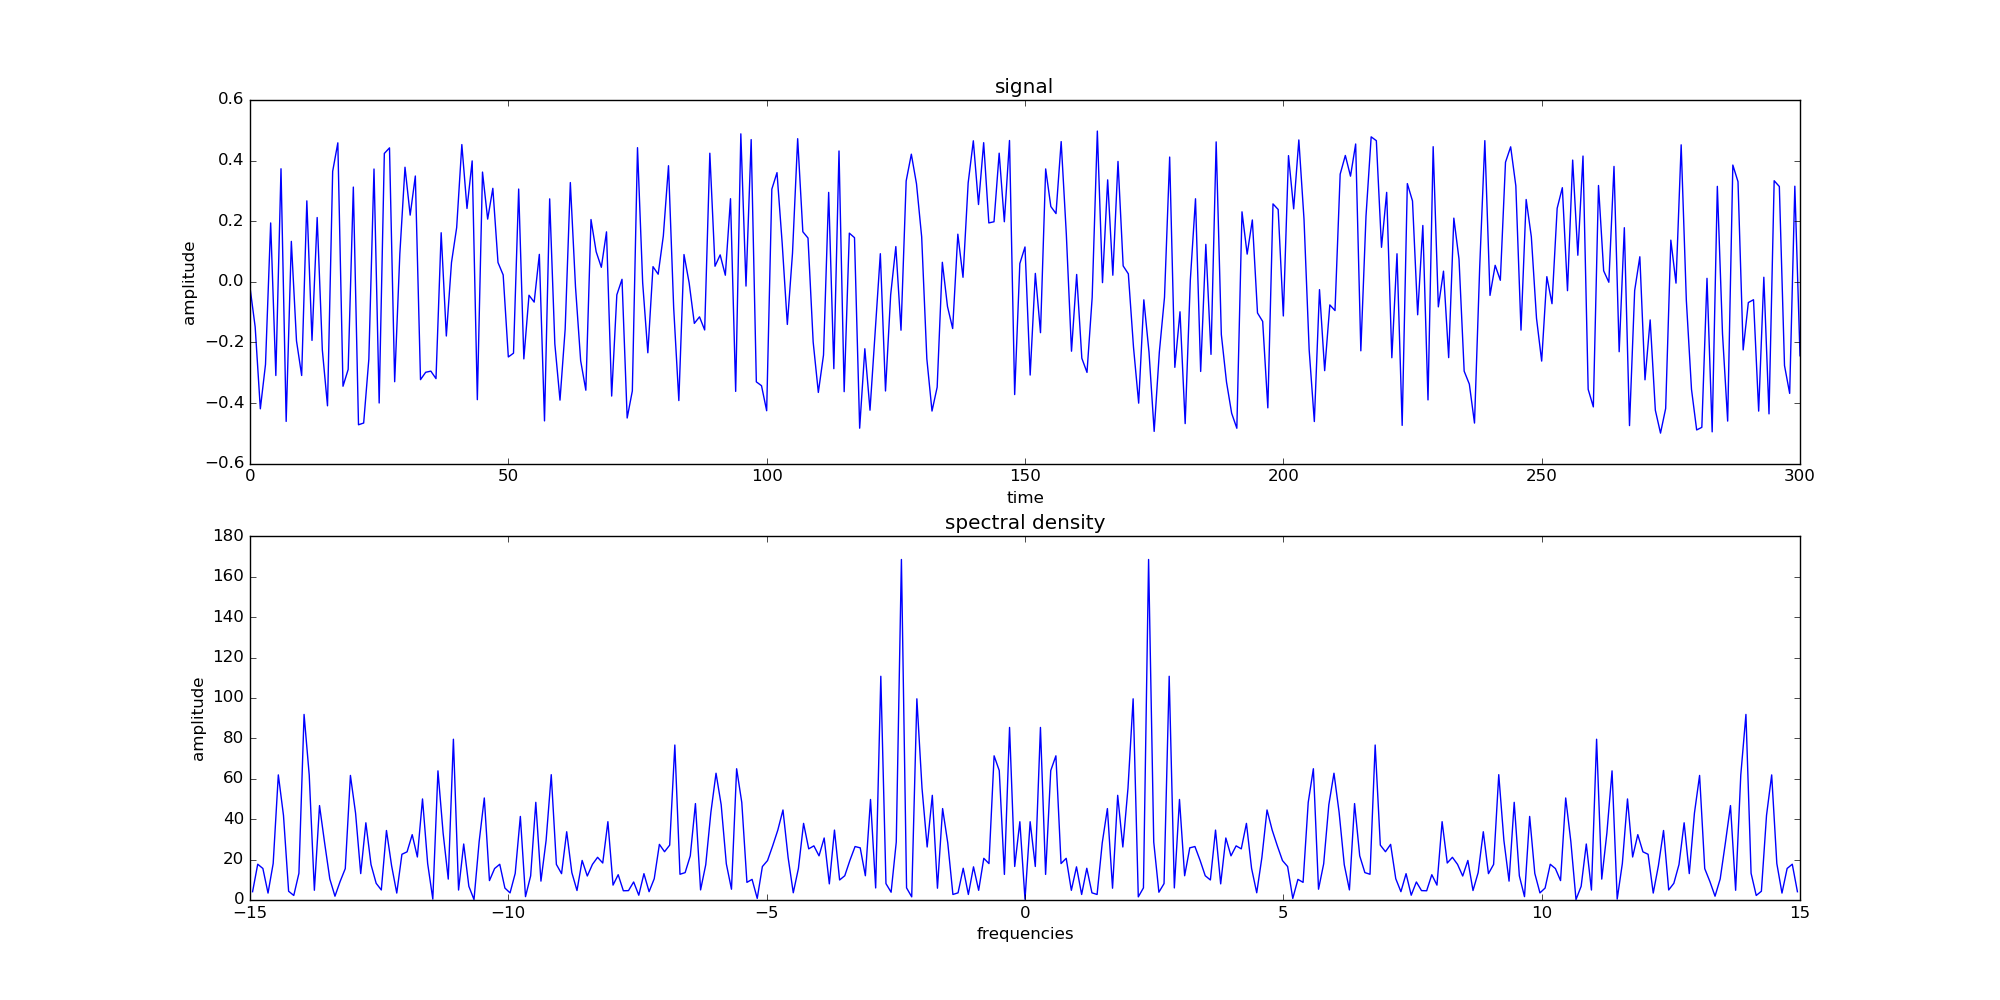
\includegraphics[width=1\textwidth]{images/spectral_density/psd}
  \caption{Plot of power spectral density (bottom) obtained after using fourier transform numpy module on the timeseries given in the topplot.\label{fig:sd_psd}}
\end{figure}

\begin{figure}[ht!]
  \centering
  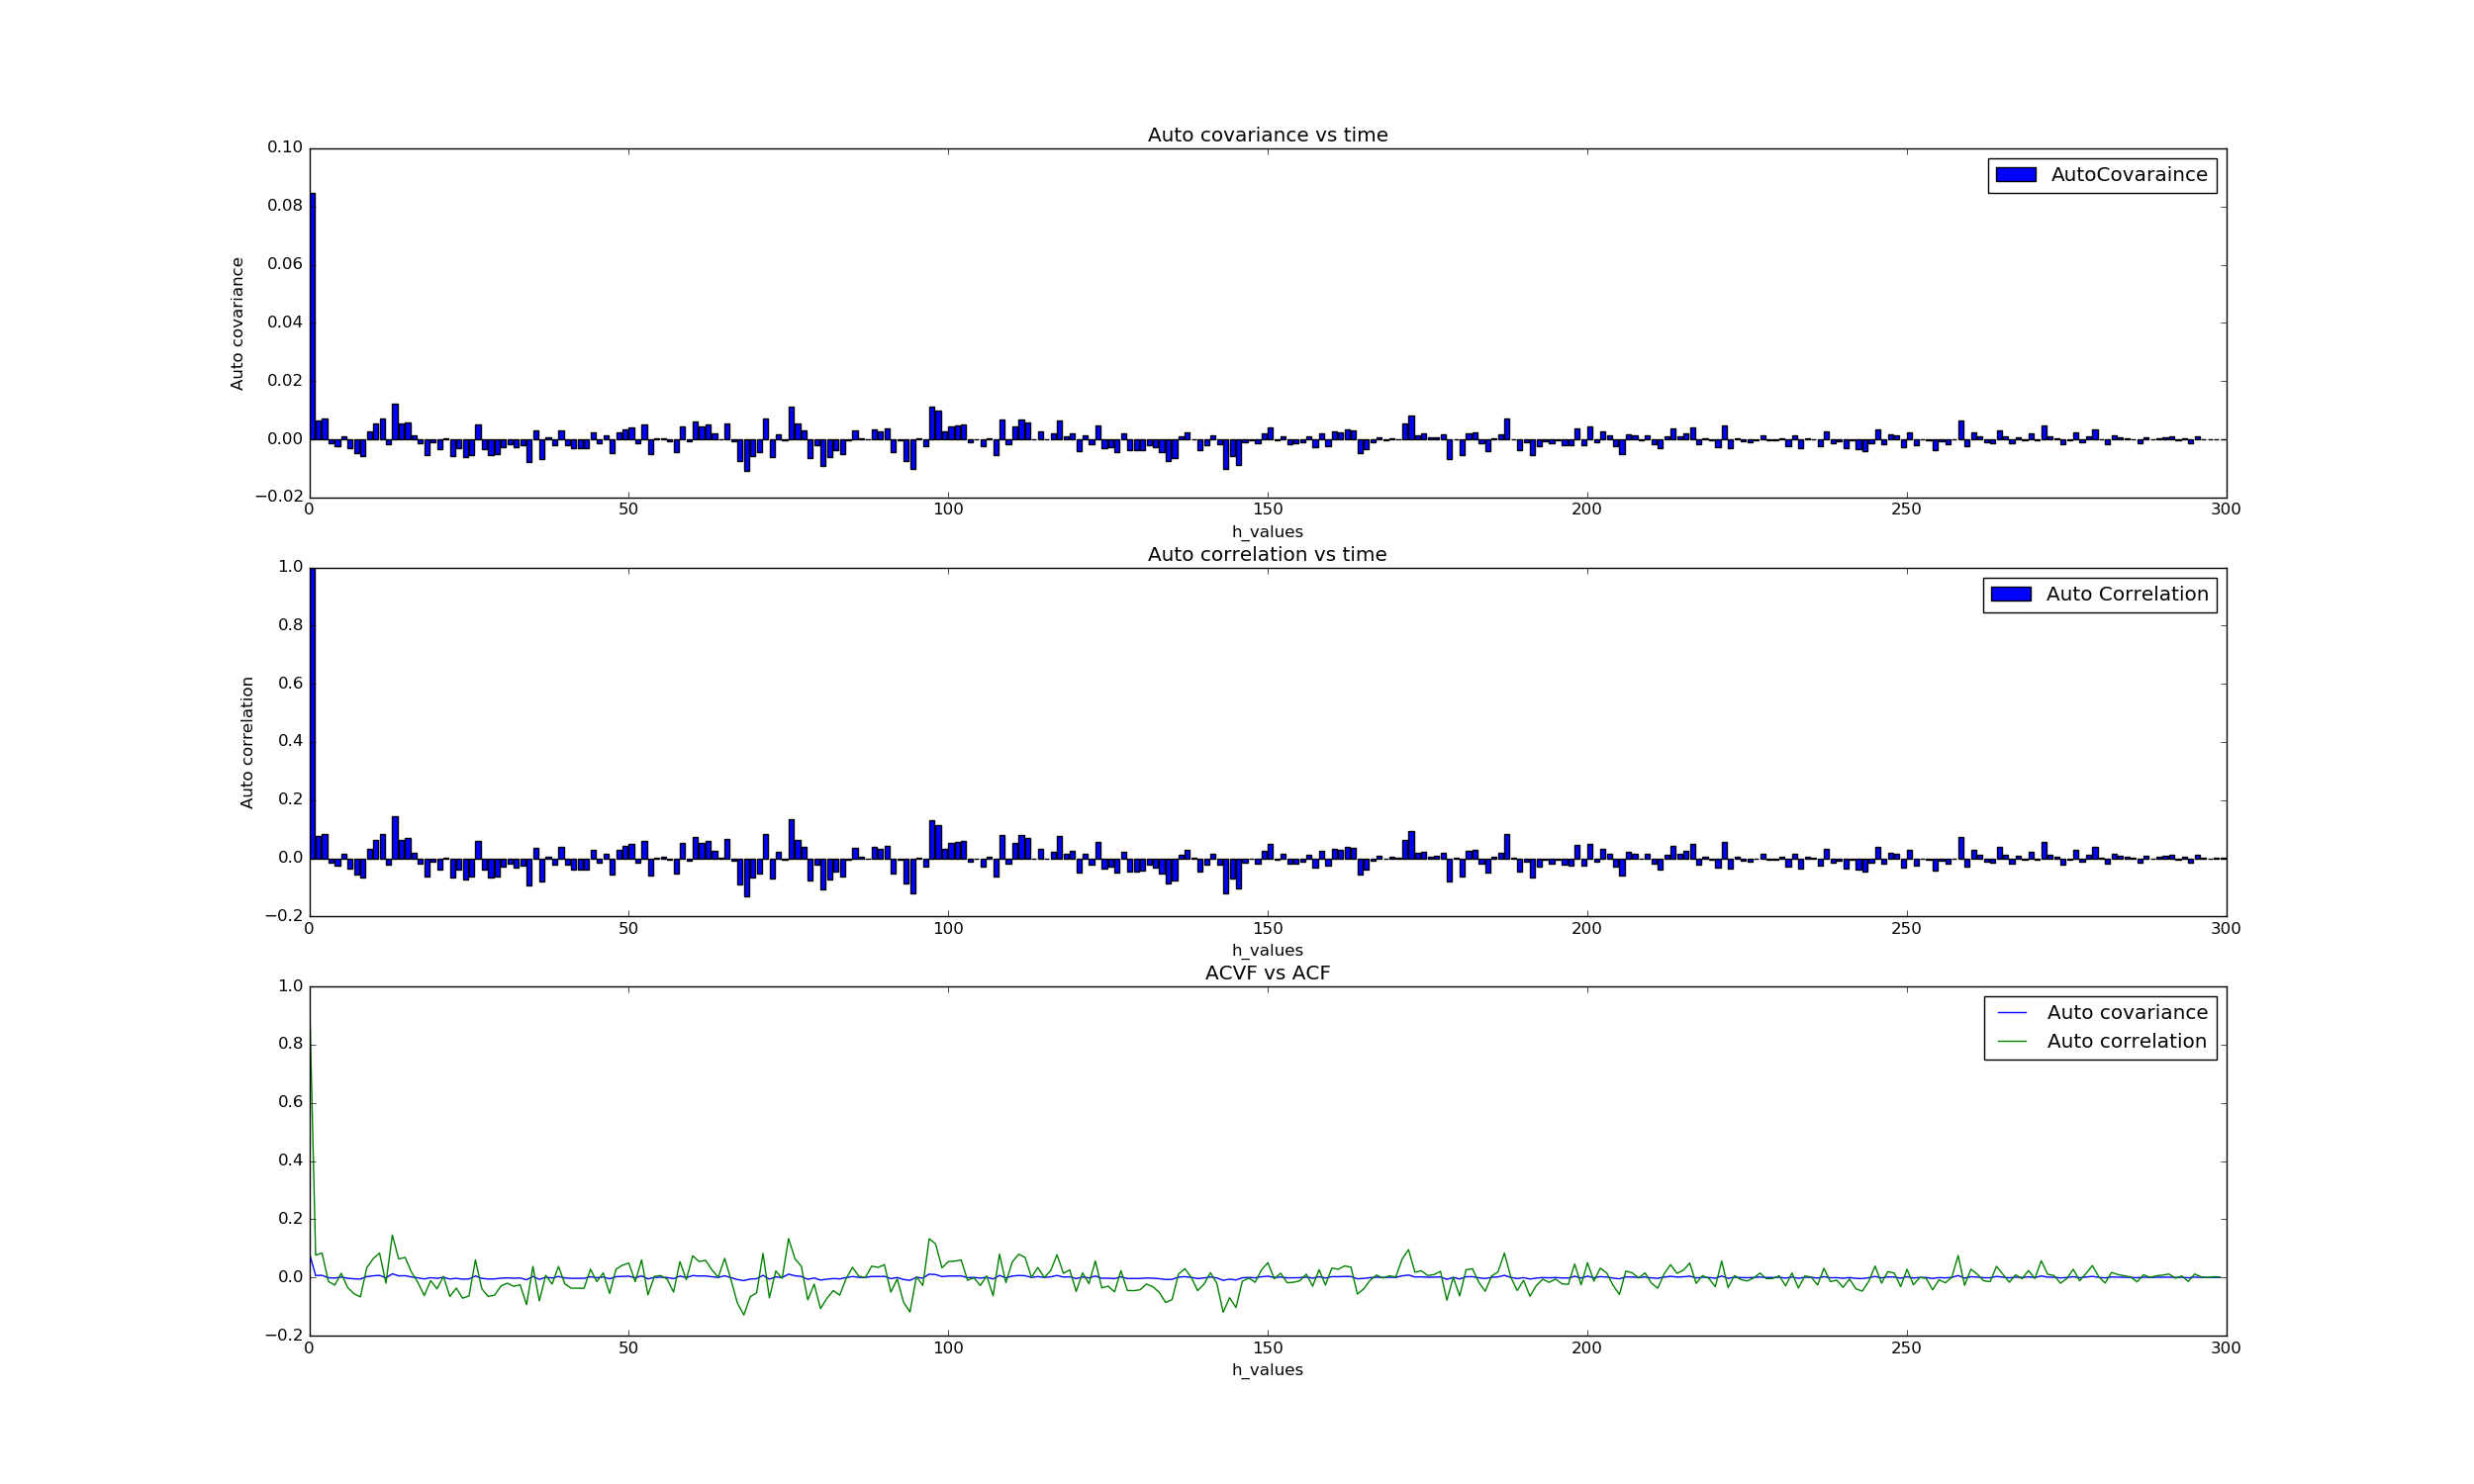
\includegraphics[width=1\textwidth]{images/spectral_density/acf_acvf}
  \caption{ACVF and ACF of the time series.\label{fig:sd_acf_acvf}}
\end{figure}

\begin{figure}[ht!]
  \centering
  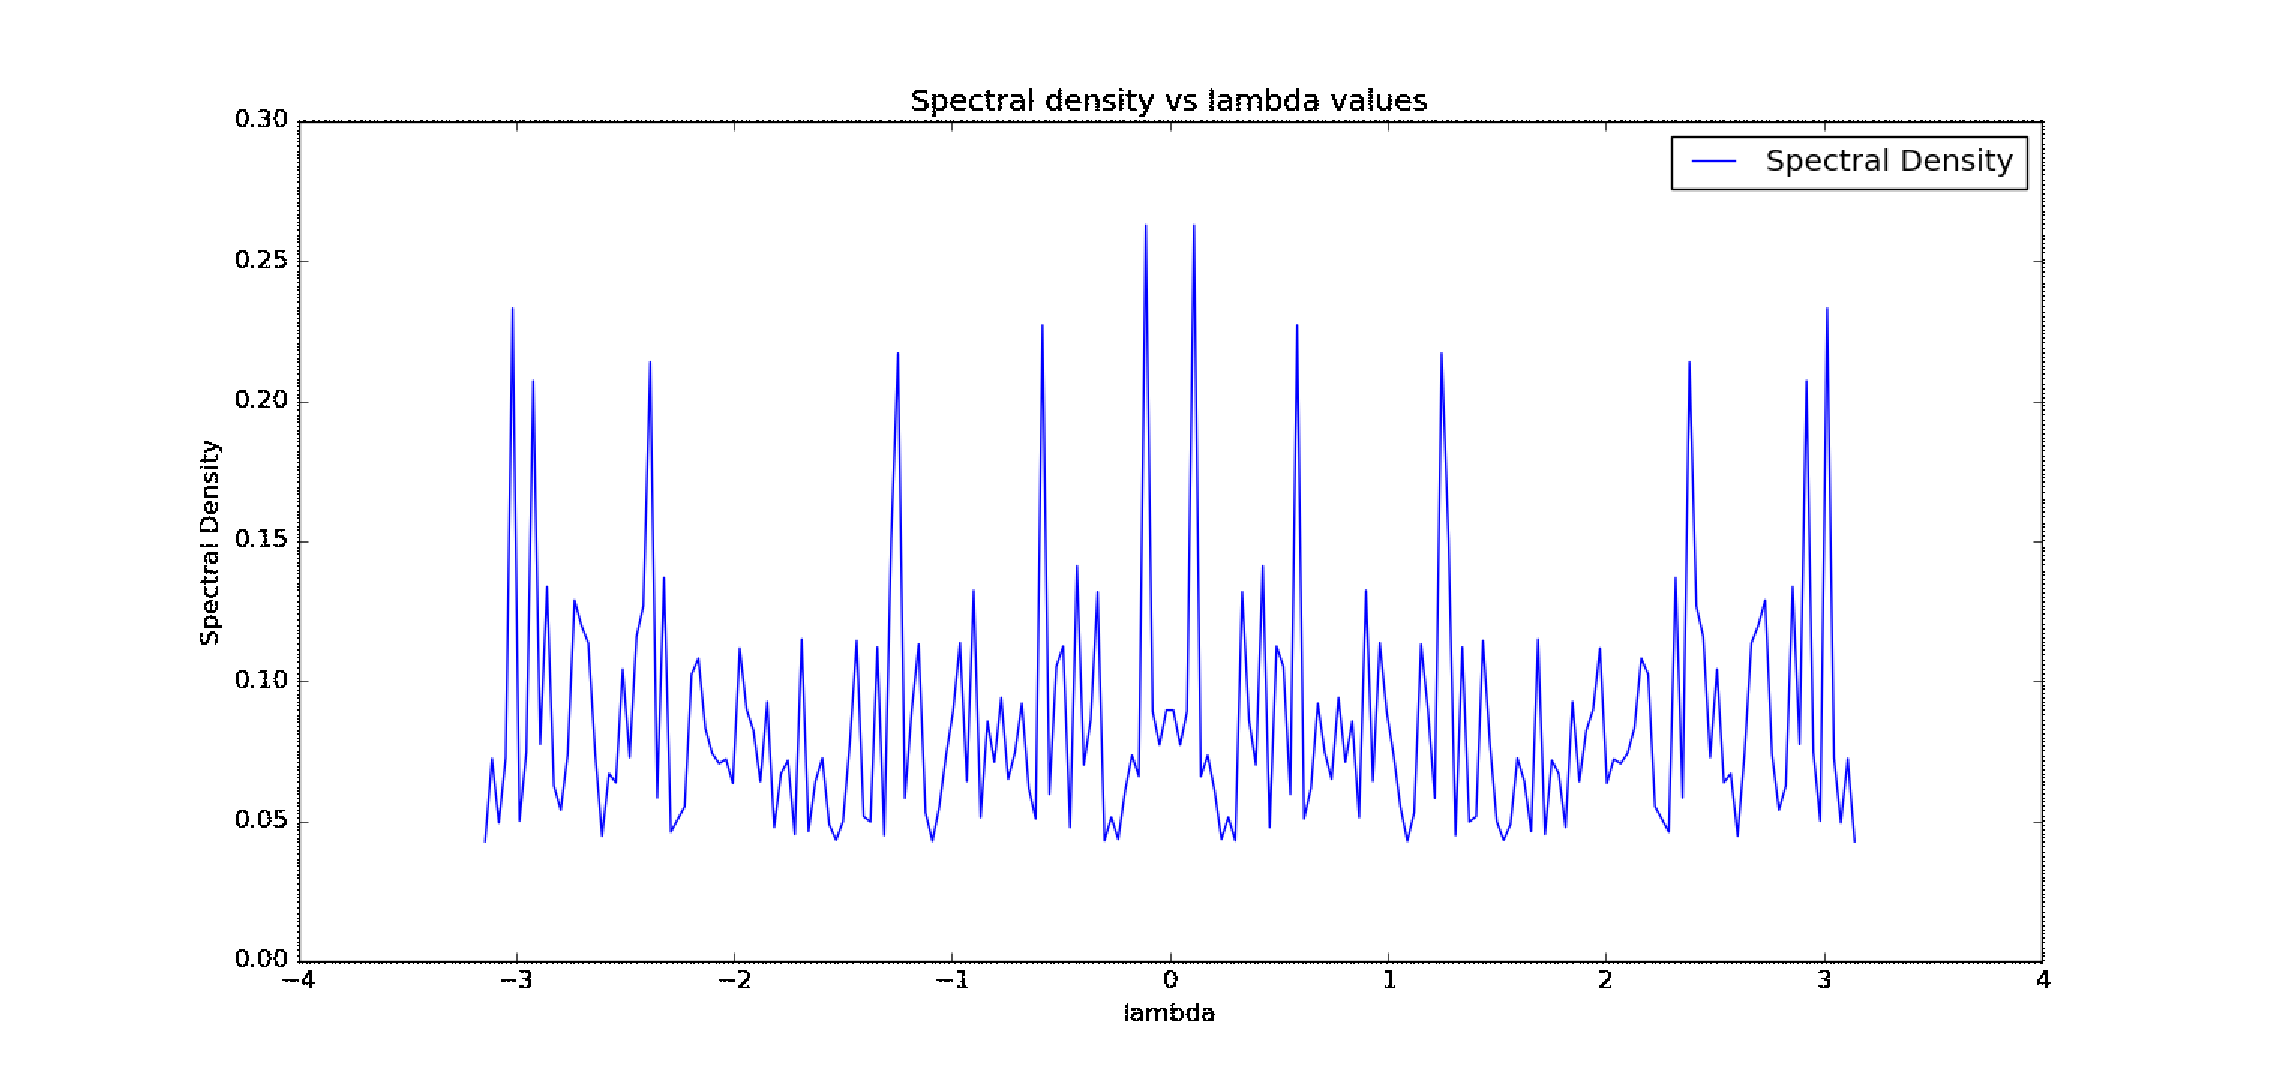
\includegraphics[width=1\textwidth]{images/spectral_density/sd}
  \caption{Spectral density for lambdas ranging from -3.14 to 3.14.\label{fig:sd_sd}}
\end{figure}

\section{Questions}
There are a number of questions I have got while working on this.
\begin{enumerate}
  \item  What exactly is the difference between Spectral Density and Power Spectral Density.
  \item  Why are we not bother about the frequency component while calculating the spectral density.
  \item  Difference between weekly stationary and strongly stationary.
\end{enumerate}

\bibliographystyle{plain}
\bibliography{references}

\end{document}
